\documentclass[UTF8,a4paper,12pt,fontset=none]{ctexart}

\usepackage{amsmath}
\usepackage{array}
\usepackage{booktabs}
\usepackage{caption}
\usepackage{enumitem}
\usepackage{fancyhdr}
\usepackage{float}
\usepackage{geometry}
\usepackage{graphicx}
\usepackage{hyperref}
\usepackage{listings}
\usepackage{longtable}
\usepackage{titlesec}
\usepackage{xcolor}
\usepackage[backend=biber,style=numeric,sorting=none]{biblatex}

\addbibresource{references.bib}
\graphicspath{{figures/}}

\definecolor{reportblue}{HTML}{1F4E79}
\definecolor{reportgray}{HTML}{586069}
\definecolor{reportlight}{HTML}{F4F7FB}

\setCJKmainfont[AutoFakeBold=2,AutoFakeSlant=.2]{Songti SC}
\setCJKsansfont[AutoFakeBold=2,AutoFakeSlant=.2]{Songti SC}
\setCJKmonofont[AutoFakeBold=2,AutoFakeSlant=.2]{Songti SC}

\geometry{left=2.65cm,right=2.65cm,top=2.85cm,bottom=2.75cm,headheight=15pt}
\hypersetup{
  colorlinks=true,
  linkcolor=blue!50!black,
  citecolor=blue!50!black,
  urlcolor=blue!50!black,
  pdftitle={类 Rust 语言编译器设计文档},
  pdfauthor={同济大学 2026 春《编译原理》课程作业}
}
\emergencystretch=2em

\pagestyle{fancy}
\fancyhf{}
\fancyhead[L]{\small 类 Rust 语言编译器设计文档}
\fancyhead[R]{\small 编译原理课程作业}
\fancyfoot[C]{\small\thepage}
\renewcommand{\headrulewidth}{0.4pt}
\renewcommand{\footrulewidth}{0pt}

\titleformat{\section}
  {\Large\bfseries\color{reportblue}}
  {\thesection}{0.8em}{}[\titlerule]
\titleformat{\subsection}
  {\large\bfseries\color{reportblue}}
  {\thesubsection}{0.8em}{}
\titleformat{\subsubsection}
  {\normalsize\bfseries\color{reportgray}}
  {\thesubsubsection}{0.8em}{}
\titlespacing*{\section}{0pt}{1.8em}{0.9em}
\titlespacing*{\subsection}{0pt}{1.1em}{0.5em}
\captionsetup{font=small,labelfont=bf,labelsep=quad}

\setlist[itemize]{leftmargin=2em,itemsep=0.2em,topsep=0.2em}
\setlist[enumerate]{leftmargin=2em,itemsep=0.2em,topsep=0.2em}

\lstdefinestyle{reportcode}{
  basicstyle=\ttfamily\small,
  columns=fullflexible,
  breaklines=true,
  frame=single,
  framerule=0.3pt,
  xleftmargin=0.5em,
  xrightmargin=0.5em,
  backgroundcolor=\color{reportlight},
  rulecolor=\color{reportblue!30}
}
\lstset{style=reportcode}

\newcommand{\code}[1]{\texttt{\detokenize{#1}}}
\newcommand{\eps}{\varepsilon}

\newcommand{\ReportTitle}{类 Rust 语言编译前端设计文档}
\newcommand{\ReportCourse}{编译原理}
\newcommand{\ReportProject}{MyRustCompiler}
\newcommand{\ReportTerm}{2026 春}

\begin{document}

\hypersetup{pageanchor=false}
\begin{titlepage}
\thispagestyle{empty}
\centering
\vspace*{1.2cm}
{\zihao{2}\bfseries 同济大学\par}
\vspace{0.6cm}
{\Large \ReportTerm《\ReportCourse》课程作业\par}
\vspace{2.0cm}
{\color{reportblue}\rule{0.78\textwidth}{1.2pt}\par}
\vspace{0.65cm}
{\zihao{1}\bfseries \ReportTitle\par}
\vspace{0.45cm}
{\large 词法分析和语法分析阶段 \par}
\vspace{0.65cm}
{\color{reportblue}\rule{0.78\textwidth}{1.2pt}\par}
\vfill
\begin{tabular}{>{\bfseries}r@{\quad}l}
项目名称 & \ReportProject \\
实现语言 & Rust \\
当前范围 & 词法分析、CLR(1) 语法分析、CST 输出 \\
姓名 & \underline{\hspace{7cm}} \\
学号 & \underline{\hspace{7cm}} \\
日期 & \today \\
\end{tabular}
\vfill
{\small 本文档依据当前源码与实测结果编写，不将尚未实现的语义分析和代码生成写作已完成功能。\par}
\end{titlepage}

\pagenumbering{Roman}
\setcounter{page}{1}

\begin{abstract}
本文档描述当前项目中已经实现并经过验证的编译前端部分。项目使用 Rust 编写，围绕一个简单类 Rust 语言完成源文件读取、词法分析、文法建模、CLR(1) 项目集族构造、ACTION/GOTO 分析表构建、表驱动语法分析以及 CST（Concrete Syntax Tree，具体语法树）输出。本文不把尚未形成源码实现的语义分析、类型检查、符号表管理和代码生成写作已完成功能，而是在不足与后续工作中如实说明。
\end{abstract}

\tableofcontents
\clearpage
\pagenumbering{arabic}
\setcounter{page}{1}
\hypersetup{pageanchor=true}

\section{实验目标与实现边界}

\subsection{实验目标}

本实验的目标是实现一个类 Rust 语言编译器前端，使其能够从源文件中识别词法单元，并依据预定义文法进行语法分析。当前实现重点放在词法分析和 CLR(1) 表驱动语法分析两个阶段，这与编译原理中经典的词法、语法前端划分一致\cite{aho2006compilers,knuth1965translation}。

结合当前源码，编译流程可以概括为：

\begin{enumerate}
  \item 读取输入文件，保存源码文本、路径和字节位置到行列号的映射。
  \item 使用词法分析器扫描源码，跳过空白和注释，生成带源代码区间的 Token 序列。
  \item 用 \code{GrammarBuilder} 构造终结符、非终结符和产生式。
  \item 计算 Nullable 集与 FIRST 集，构造 LR(1) 项目集族。
  \item 根据项目集族生成 ACTION/GOTO 分析表。
  \item 解析 Token 序列，执行移进、规约和接受动作，同时构造 CST。
  \item 输出编译成功信息，必要时以文本形式展示 CST。
\end{enumerate}

\subsection{实现边界}

当前项目名为 \code{MyRustCompiler}，但源码中已经落地的部分是编译前端。README 中提到语义分析和代码生成方向，但在当前源码中没有可验证的语义分析器、符号表、类型检查器或目标代码生成器。因此，本文档仅把这些内容作为后续工作，不将其计入已实现功能。

当前命令行入口位于 \code{src/main.rs}。程序通过 \code{clap} 解析参数，支持 \code{--rebuild} 强制重建前端缓存，支持 \code{--verbose} 输出 CST，当前默认只处理参数列表中的第一个源文件。项目依赖 \code{clap}、\code{serde} 和 \code{serde-binary-adv}，分别用于命令行参数、结构序列化以及前端缓存的二进制读写\cite{clap-docs,serde-docs,serde-binary-adv-docs}。

\section{问题分析}

\subsection{词法分析问题}

词法分析的任务是从字符流中切分出有语法意义的 Token。该项目的词法分析器位于 \code{src/lexer.rs}，底层游标位于 \code{src/lexer/cursor.rs}，Token 类型定义位于 \code{src/lexer/token.rs}。词法分析器需要解决以下问题：

\begin{itemize}
  \item 跳过空白字符、行注释和块注释，其中块注释支持嵌套。
  \item 区分关键字和普通标识符。
  \item 识别目前只支持的 \code{i32} 整数字面量。
  \item 识别单字符和双字符运算符，例如 \code{+}、\code{-}、\code{==}、\code{<=}、\code{!=}。
  \item 识别界符、分隔符和特殊符号，例如括号、逗号、分号、\code{->}、\code{..}。
  \item 对无法识别的字符返回 \code{Error} Token。
\end{itemize}

源码中的扫描顺序是：先跳过 trivia，再依次尝试特殊符号、标识符或关键字、数字、运算符或赋值、界符、分隔符。这个顺序保证了 \code{->} 优先被识别为特殊符号，而不是先被识别成 \code{-}；也保证了 \code{..} 采用最长匹配。

\begin{figure}[H]
\centering
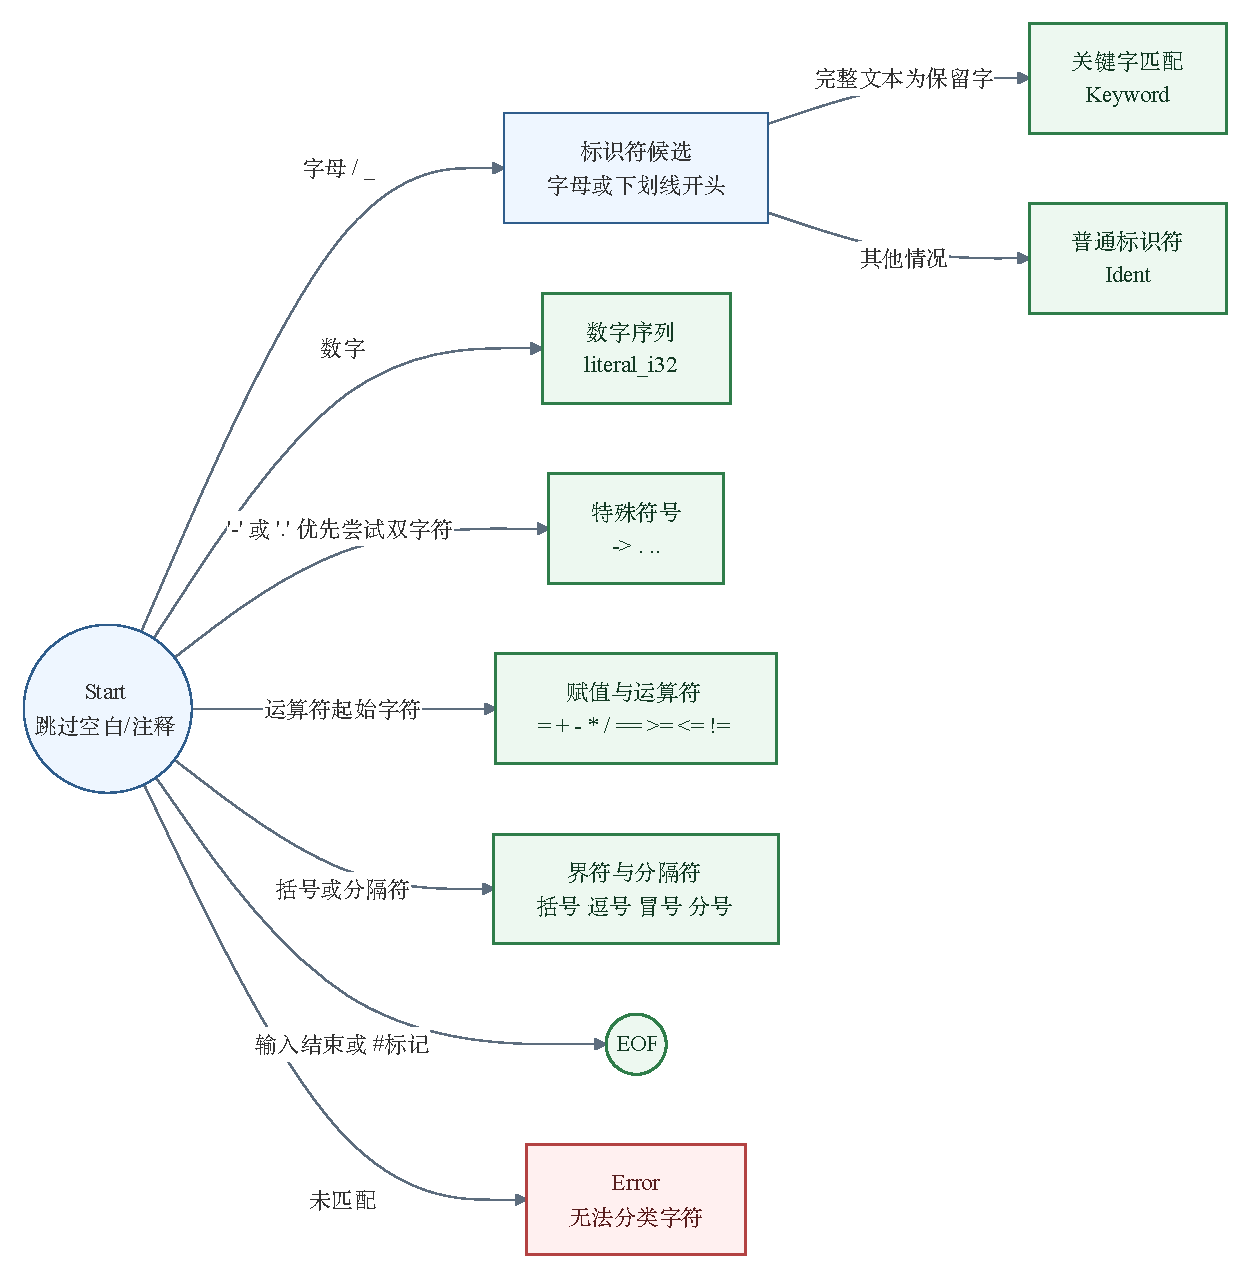
\includegraphics[width=0.94\textwidth]{lexer-fsm.pdf}
\caption{词法分析状态转换示意图}
\label{fig:lexer-fsm}
\end{figure}

\subsection{语法分析问题}

语法分析的任务是根据 Token 序列判断程序是否满足文法，并构造反映语法结构的树。该项目采用正规 LR(1)，即 CLR(1) 表驱动分析。LR(1) 项目形如：

\[
  [A \rightarrow \alpha \cdot \beta, a]
\]

其中点号表示当前识别进度，向前看符号 \(a\) 用于判断规约是否可执行。相比简单自顶向下分析，LR(1) 更适合处理左递归表达式文法，例如项目中用于表达式优先级的规则：

\[
\begin{aligned}
  \langle expr\rangle &\rightarrow \langle expr\rangle \ \langle cmp\_op\rangle \ \langle add\_expr\rangle \\
  \langle add\_expr\rangle &\rightarrow \langle add\_expr\rangle \ \langle add\_op\rangle \ \langle term\rangle \\
  \langle term\rangle &\rightarrow \langle term\rangle \ \langle mul\_op\rangle \ \langle factor\rangle
\end{aligned}
\]

分析器需要在运行前根据文法生成 ACTION/GOTO 表，运行时只依赖状态栈、节点栈、当前输入 Token 和分析表完成判断。

\section{系统总体设计}

\subsection{模块结构}

当前系统可以分为源文件管理、词法分析、文法与分析表构建、语法分析执行、输出展示五个部分。总体结构如图~\ref{fig:module-structure} 所示。

\begin{figure}[H]
\centering
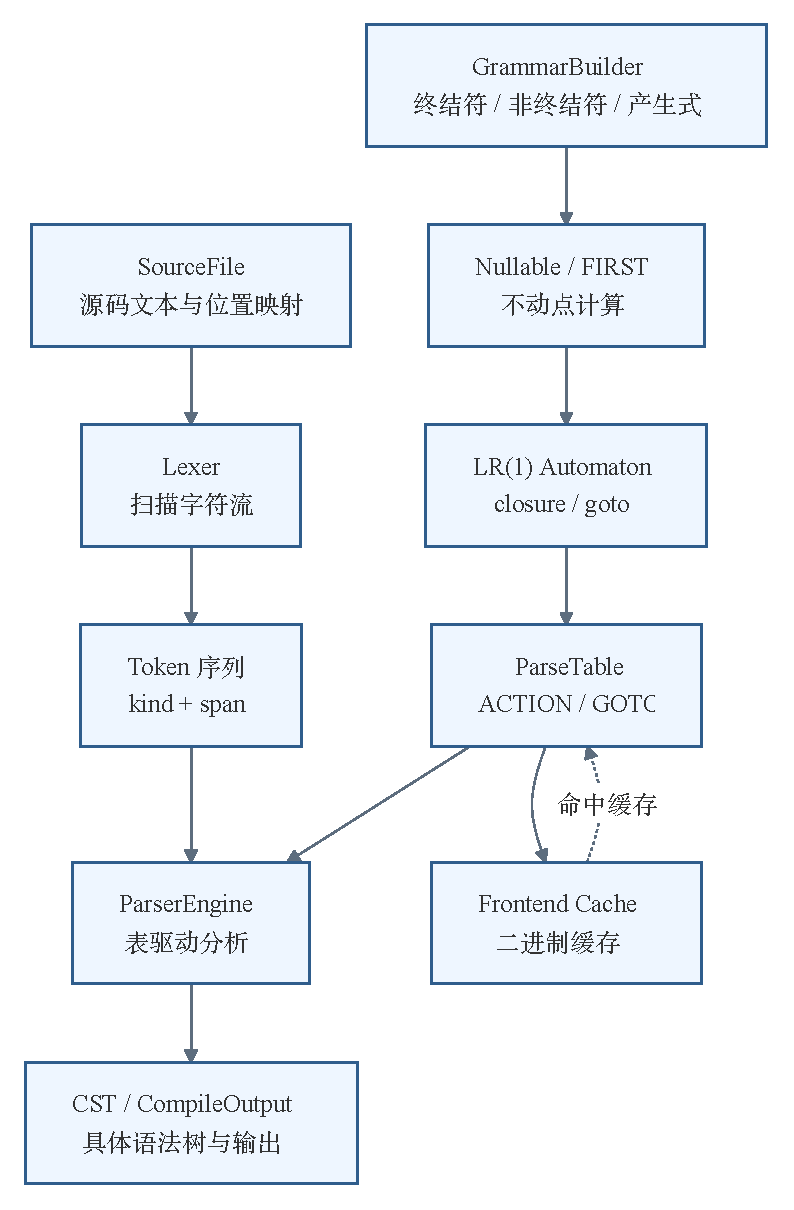
\includegraphics[width=0.9\textwidth,height=0.42\textheight,keepaspectratio]{module-structure.pdf}
\caption{系统模块结构图}
\label{fig:module-structure}
\end{figure}

\subsection{核心数据流}

\code{Compiler::compile} 是前端主流程。它先通过 \code{Lexer} 遍历源码并收集普通 Token，再在源码末尾补充 \code{Eof} Token。随后创建 \code{ParserEngine}，传入前端缓存中的 \code{ParseTable} 和 \code{GrammarContext}，最终返回 \code{CompileOutput}。

\code{Compiler::build} 负责前端初始化。它先通过 \code{generate_my_grammar_context} 构造文法上下文，再根据文法序列化结果和缓存版本计算缓存键。如果缓存存在且未要求重建，就直接加载；否则重新构造 Nullable/FIRST、LR(1) 自动机和分析表，并写入 \code{cache/frontend/}。

\section{详细设计}

\subsection{源文件与游标}

\code{SourceFile} 保存源码文本、可选路径和每行起始字节位置。它提供源码切片、行列号换算和行文本读取等辅助方法，为后续诊断输出和 CST span 展示提供基础。当前 CST span 使用字节区间，因此 \code{Cursor} 的位置也采用 UTF-8 字节偏移。

\code{Cursor} 基于 Rust 标准库的 \code{CharIndices} 实现，提供 \code{peek}、\code{peek_next}、\code{bump}、\code{eat_if} 和 \code{eat_while}。这种设计避免手动处理 UTF-8 字符宽度，源码中也有单测验证中文标识符时字节偏移能够正确推进。字符分类依赖 Rust 标准库的 \code{char} 方法，例如 \code{is_alphabetic}、\code{is_alphanumeric} 和 \code{is_numeric}\cite{rust-std-char}。

\subsection{Token 分类与词法规则}

Token 包含 \code{TokenKind} 和 \code{Span} 两部分。当前实现的 Token 种类如表~\ref{tab:token-kind} 所示。

\begin{longtable}{p{0.24\textwidth}p{0.66\textwidth}}
\caption{Token 分类}\label{tab:token-kind}\\
\toprule
类别 & 实际内容 \\
\midrule
\endfirsthead
\toprule
类别 & 实际内容 \\
\midrule
\endhead
关键字 & \code{i32}、\code{let}、\code{if}、\code{else}、\code{while}、\code{return}、\code{mut}、\code{fn}、\code{for}、\code{in}、\code{loop}、\code{break}、\code{continue} \\
标识符 & 字母或下划线开头，后续可包含字母、数字或下划线；根据 Rust \code{char} 分类函数，源码中可接受 UTF-8 字母字符。 \\
字面量 & 当前只支持 \code{i32} 整数字面量，即连续数字。 \\
赋值与运算符 & \code{=}、\code{+}、\code{-}、\code{*}、\code{/}、\code{==}、\code{>}、\code{>=}、\code{<}、\code{<=}、\code{!=}、\code{\&}。 \\
界符 & \code{(}、\code{)}、\code{\{}、\code{\}}、\code{[}、\code{]}。 \\
分隔符 & \code{;}、\code{:}、\code{,}。 \\
特殊符号 & \code{->}、\code{.}、\code{..}。 \\
结束与错误 & \code{Eof} 和 \code{Error}。源码中 \code{\#} 也被视为 EOF 标记。 \\
\bottomrule
\end{longtable}

词法分析采用一组局部解析函数组合而成。对于可能为单字符或双字符的符号，统一使用 \code{lex_one_or_two_char_token}：先尝试两个字符的分类，成功则消费两个字符；否则尝试一个字符，成功则消费一个字符；两者都失败时不消费字符并返回 \code{None}。该策略用于 \code{==}、\code{>=}、\code{<=}、\code{!=}、\code{->} 和 \code{..} 等最长匹配场景。

注释处理位于 \code{skip_comment}。行注释从 \code{//} 开始直到换行前结束；块注释从 \code{/*} 开始到匹配的 \code{*/} 结束，并通过 \code{depth} 计数支持嵌套块注释。

\subsection{文法建模}

文法构造集中在 \code{src/my_grammar.rs}。源码定义阶段添加了 40 个终结符、46 个非终结符和 107 条业务产生式；\code{GrammarBuilder::build} 会自动添加扩展起始符号和扩展起始产生式，因此构造后的文法还包含一个额外的增广起始产生式。

\code{Grammar} 结构保存：

\begin{itemize}
  \item \code{terminals}：终结符表。
  \item \code{non_terminals}：非终结符表。
  \item \code{productions}：产生式数组，每条产生式包含左部非终结符和右部符号序列。
  \item \code{start}：用户文法起始符号。
  \item \code{augmented_start}：自动添加的扩展起始符号。
  \item \code{eof}：文件结束终结符。
\end{itemize}

当前文法按语言特性逐步扩展：基础程序、变量声明、赋值语句、表达式、选择结构、循环结构、引用、块表达式、数组和元组。表达式文法使用左递归表达优先级，其中乘除优先级高于加减，加减高于比较。

\subsection{Nullable 与 FIRST 集}

\code{NullableSet::compute} 通过不动点迭代计算每个非终结符是否能推出空串。若产生式右部为空，或者右部所有非终结符都可空，则左部可空。

\code{FirstSets::compute} 同样采用不动点迭代。对每条产生式 \(A \rightarrow X_1 X_2 \cdots X_n\)，从左到右扫描右部符号：

\begin{itemize}
  \item 遇到终结符 \(t\)，将 \(t\) 加入 FIRST(\(A\)) 并停止。
  \item 遇到非终结符 \(B\)，将 FIRST(\(B\)) 加入 FIRST(\(A\))；若 \(B\) 不可空，则停止。
\end{itemize}

LR(1) closure 需要计算 \(\mathrm{FIRST}(\beta a)\)。源码中 \code{first_of_sequence} 将项目点后剩余符号序列与 lookahead 拼接，再按 FIRST 规则求首终结符集合。

\subsection{CLR(1) 项目集族构造}

LR(1) 项目由 \code{Lr1Item} 表示，核心字段是产生式编号、点号位置和向前看终结符。项目集由 \code{ItemSet} 表示，内部使用 \code{BTreeSet} 去重和排序。

\code{Automaton::closure_} 的逻辑如下：

\begin{enumerate}
  \item 将输入项目加入闭包集合和队列。
  \item 从队列取出项目，若点号后是非终结符 \(B\)，则计算点号后继序列和 lookahead 的 FIRST 集。
  \item 对 \(B\) 的每条产生式 \(B \rightarrow \gamma\)，以及 FIRST 集中每个向前看符号 \(b\)，加入新项目 \([B \rightarrow \cdot \gamma, b]\)。
  \item 若新项目此前未出现，则继续入队扩展。
\end{enumerate}

\code{Automaton::goto_} 先收集所有点号后为目标符号 \(X\) 的项目，并将点号前进一位，然后对结果求 closure。完整项目集族从增广起始项目开始，用队列广度优先展开所有可达状态。

\begin{figure}[H]
\centering
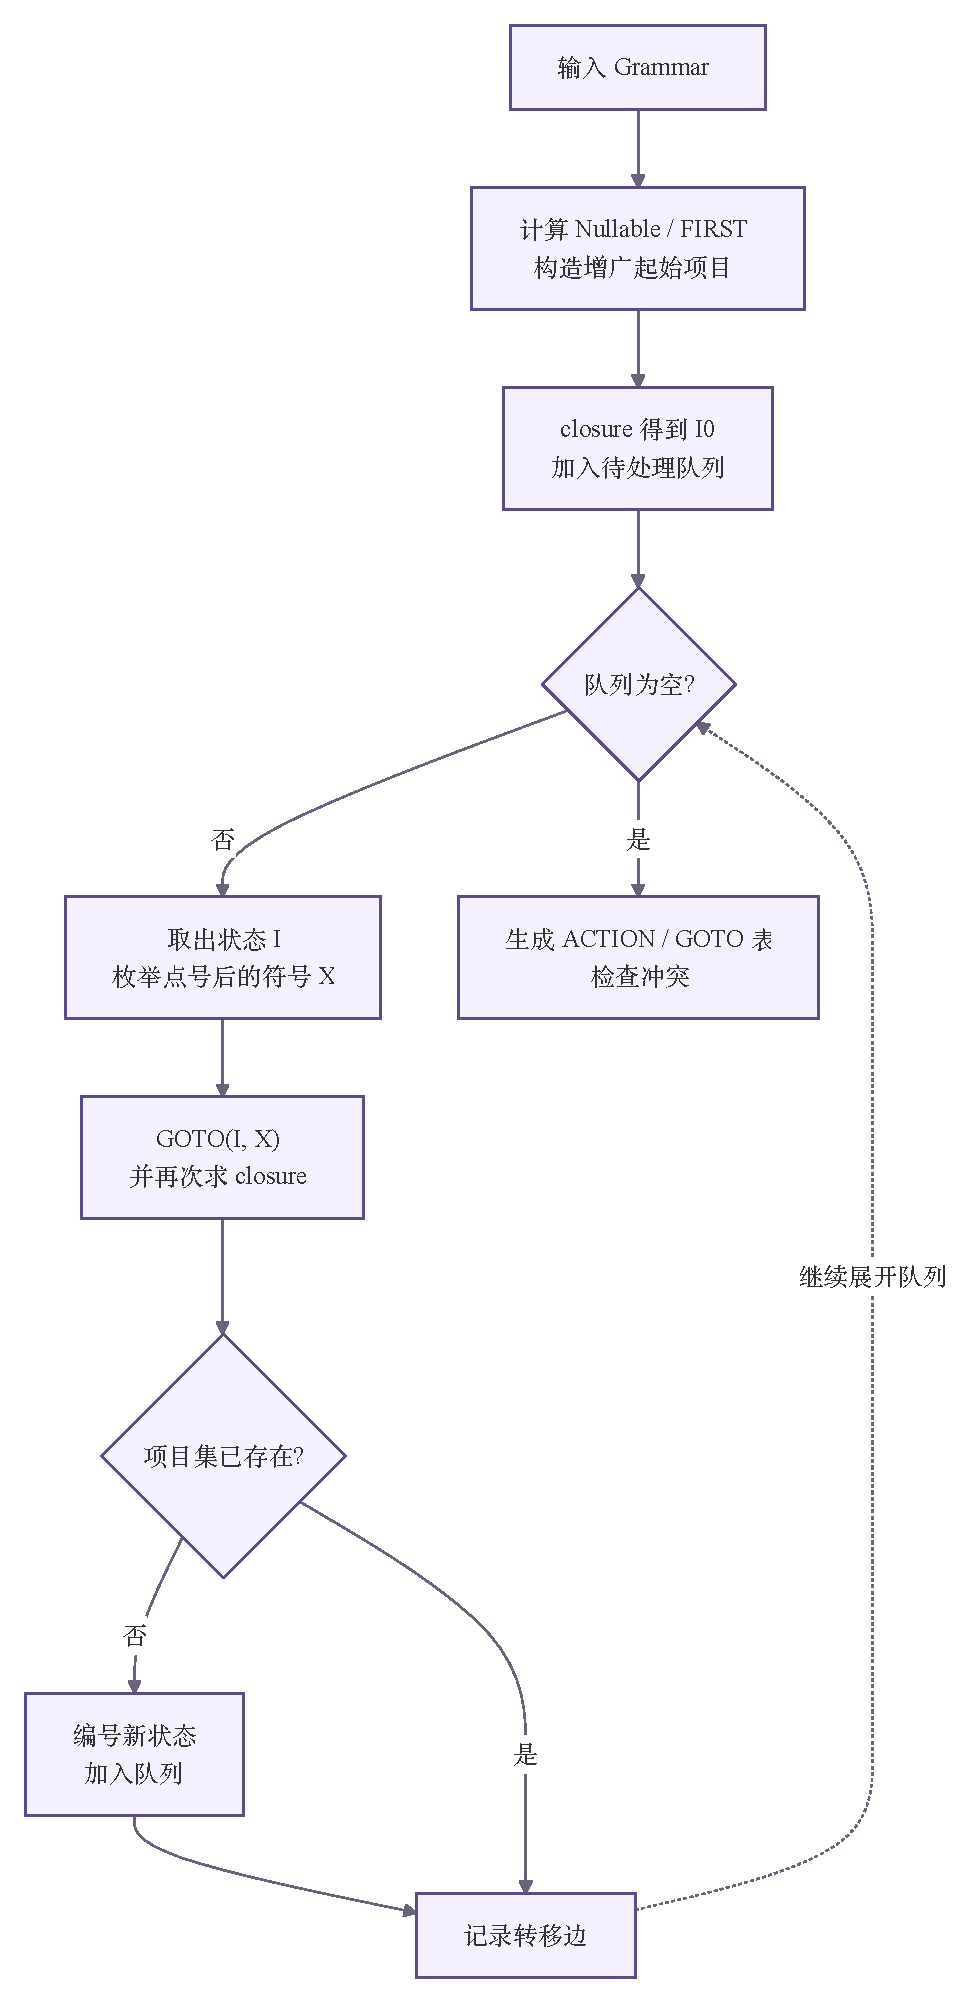
\includegraphics[width=0.92\textwidth,height=0.64\textheight,keepaspectratio]{clr-flow.pdf}
\caption{CLR(1) 构表流程图}
\label{fig:clr-flow}
\end{figure}

\subsection{ACTION/GOTO 分析表}

\code{ParseTable} 由两个映射组成：

\[
  ACTION: (StateID, TerminalId) \rightarrow Action
\]

\[
  GOTO: (StateID, NonTerminalId) \rightarrow StateID
\]

\code{Action} 包含三类动作：

\begin{itemize}
  \item \code{Shift(StateID)}：读入当前终结符并转移到新状态。
  \item \code{Reduce(ProductionId)}：按照指定产生式规约。
  \item \code{Accept}：接受输入。
\end{itemize}

构表分两步进行：先根据自动机转移边填入 shift 和 goto；再遍历每个状态中的规约项目，在该项目 lookahead 对应的 ACTION 单元填入 reduce 或 accept。若同一表项出现不同动作，源码会返回移进/规约冲突、规约/规约冲突或非法 GOTO 错误。

\subsection{表驱动语法分析与 CST 构造}

\code{ParserEngine::parse} 维护两个栈：

\begin{itemize}
  \item 状态栈：初始为 \code{StateID(0)}。
  \item 节点栈：保存已经构造的 CST 节点编号。
\end{itemize}

每次根据状态栈栈顶和当前输入 Token 映射出的终结符查 ACTION 表。若动作为 shift，则创建 Token 节点，将目标状态压栈并读入下一个 Token；若动作为 reduce，则弹出产生式右部长度个状态和节点，构造一个规则节点，再根据 GOTO 表压入新状态；若动作为 accept，则将节点栈顶设为 CST 根节点并返回成功。

\begin{figure}[H]
\centering
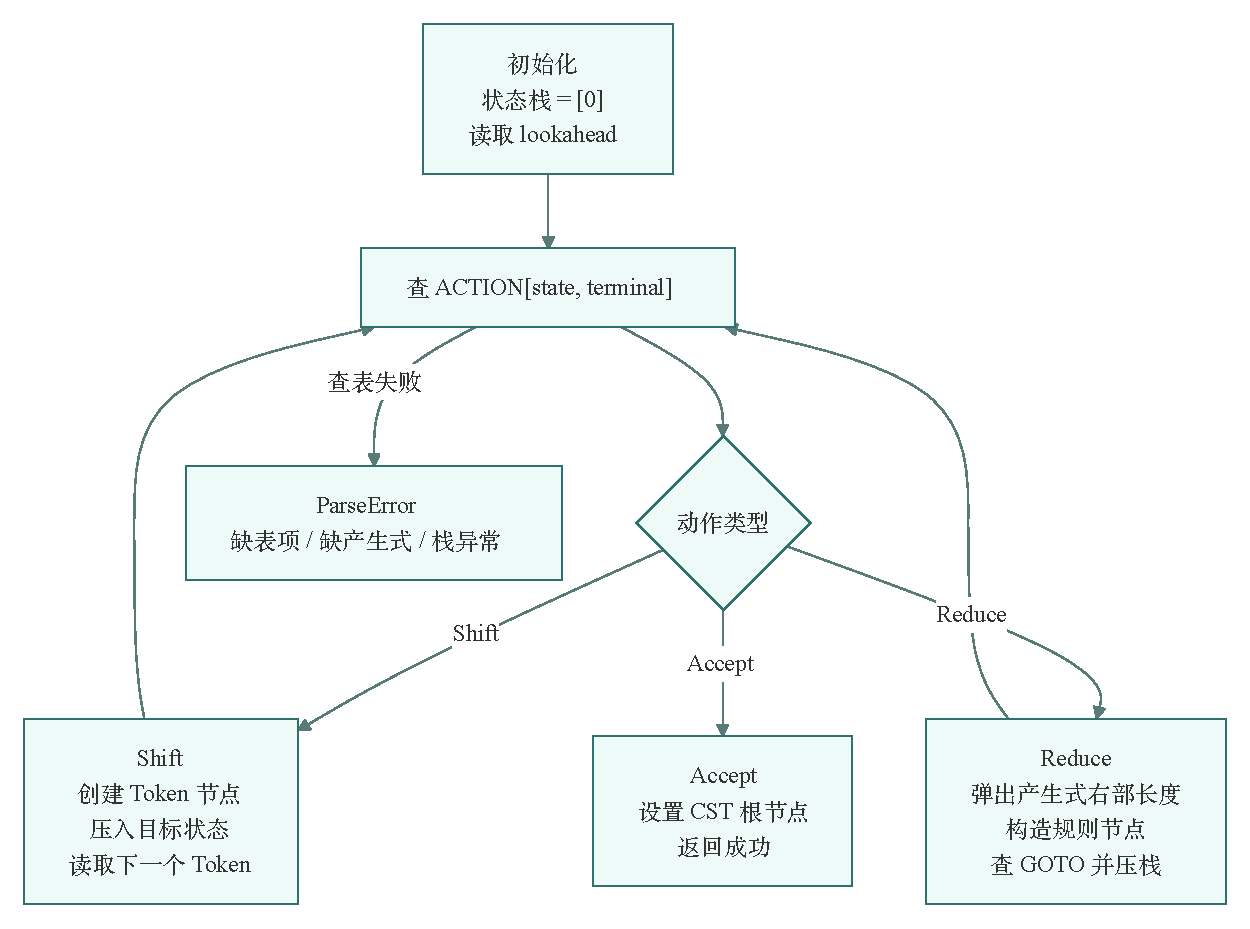
\includegraphics[width=0.76\textwidth]{parser-flow.pdf}
\caption{表驱动语法分析流程图}
\label{fig:parser-flow}
\end{figure}

CST 节点分为 \code{CSTTokenNode} 和 \code{CSTRuleNode}。Token 节点保存终结符 ID 和源码 span；规则节点保存非终结符 ID、产生式 ID、子节点列表和覆盖区间。空产生式规约时没有子节点，源码使用当前 lookahead 的起始位置构造零长度 span。

\subsection{前端缓存}

构建 LR(1) 项目集族和分析表的成本高于普通解析过程，因此 \code{Compiler} 增加了前端缓存。缓存键由文法上下文的二进制序列化结果、缓存 schema 版本和哈希值共同决定。缓存文件位于 \code{cache/frontend/}，内容包括 \code{GrammarContext} 和 \code{ParseTable}。

当命令行没有指定 \code{--rebuild} 且缓存可读时，编译器直接加载前端缓存；否则重新构建并写回缓存。该设计让文法稳定时的日常测试和示例运行更快，同时在文法变更后仍可通过强制重建避免旧表干扰。

\section{文法与功能范围}

\subsection{当前支持的语言结构}

根据 \code{src/my_grammar.rs} 中实际产生式，当前语言支持如下语法结构：

\begin{itemize}
  \item 函数声明：支持 \code{fn id(...)}，可选 \code{-> i32} 或引用类型等返回类型。
  \item 参数列表：支持空参数、单参数和逗号分隔参数；参数可带 \code{mut}。
  \item 语句块：支持普通语句块和可作为表达式的块。
  \item 变量声明与初始化：支持 \code{let x;}、\code{let mut x:i32;}、\code{let x = expr;}。
  \item 赋值语句：支持左值赋值，例如 \code{x = expr;} 和 \code{*p = expr;}。
  \item 返回语句：支持 \code{return;} 和 \code{return expr;}。
  \item 表达式：支持整数、左值、括号表达式、函数调用、比较、加减、乘除。
  \item 选择结构：支持 \code{if}、\code{else} 和 \code{else if}。
  \item 循环结构：支持 \code{while}、\code{for x in a..b}、\code{loop}。
  \item 跳转语句：支持 \code{break;}、\code{break expr;} 和 \code{continue;}。
  \item 引用相关：支持 \code{\&T}、\code{\&mut T}、\code{\&x}、\code{\&mut x} 和 \code{*x}。
  \item 数组：支持数组类型、数组表达式和下标访问。
  \item 元组：支持元组类型、元组表达式和点号访问。
\end{itemize}

\subsection{示例程序覆盖}

\code{example_source/source1.txt} 是当前项目中的综合示例。它覆盖了函数调用、表达式返回函数体、可变引用、解引用赋值、嵌套 if/else、块表达式、if 表达式、loop 表达式、数组、元组、for 循环、while 循环、break/continue、行注释和嵌套块注释。该示例可以作为本文实验验证的主样例。

\section{实验验证}

\subsection{单元测试结果}

在项目根目录运行：

\begin{lstlisting}[language=bash]
cargo test
\end{lstlisting}

当前结果为 108 个测试全部通过，0 个失败。测试覆盖范围包括：

\begin{itemize}
  \item \code{Cursor} 的前进、查看、条件消费和 UTF-8 字节偏移。
  \item 关键字、标识符、整数、运算符、特殊符号、界符、分隔符的词法识别。
  \item 空白、行注释、块注释和嵌套块注释跳过逻辑。
  \item Nullable/FIRST 集计算。
  \item LR(1) closure、goto 和项目集族构造。
  \item 表驱动分析中的 shift、reduce、accept 和错误路径。
  \item 源文件位置映射、编译输出和 CST 展示模式。
\end{itemize}

测试输出中存在少量未使用函数或枚举的 warning，例如 \code{generate_my_grammar}、\code{GrammarError} 等未使用提示。这些 warning 不影响当前词法和语法分析结果，但说明后续仍可清理未使用接口。

\subsection{综合样例运行结果}

在项目根目录运行：

\begin{lstlisting}[language=bash]
cargo run -- example_source/source1.txt
\end{lstlisting}

当前结果为编译前端构建成功、从缓存加载前端，并成功解析示例文件：

\begin{lstlisting}
Compile succeeded. CST has 1456 nodes.
\end{lstlisting}

使用详细输出模式：

\begin{lstlisting}[language=bash]
cargo run -- --verbose example_source/source1.txt
\end{lstlisting}

可以打印 CST。CST 中每个规则节点对应一个非终结符，每个叶子 Token 节点对应一个终结符，并带有源码字节区间。该输出说明当前 ParserEngine 不只是判断输入是否合法，还能保留具体语法结构，便于后续语义分析阶段继续使用。

\section{不足与个人思考}

\subsection{当前不足}

当前项目已经完成了编译前端的主要骨架，但仍存在以下边界：

\begin{itemize}
  \item 尚未实现语义分析、类型检查、符号表管理和代码生成，因此无法判断变量是否声明、类型是否匹配，也不能生成中间代码或目标代码。
  \item 语法错误处理较基础。当前主要返回缺失 ACTION、缺失 GOTO、意外 Token 等错误，没有实现同步点恢复和面向用户的详细诊断。
  \item 命令行入口当前只处理传入路径列表中的第一个文件。
  \item 词法错误 Token 的 span 是零长度区间，后续可改为消费未知字符并给出更直观的位置。
  \item 文法中部分变量命名如 \code{l_brace}/\code{l_bracket} 与具体符号映射存在容易混淆的地方，虽然运行时通过映射保持一致，但文档和后续维护需要特别注意。
\end{itemize}

\subsection{个人思考}

本项目选择先实现表驱动 CLR(1) 分析器，而不是直接为每种语法手写递归下降函数。这样做的优点是文法、项目集、分析表和运行时解析过程分离得比较清楚，能够直接对应课堂中的 LR 分析理论，也便于观察 FIRST、closure、goto、ACTION/GOTO 等算法的实际作用。

同时，这种设计也带来了更高的工程复杂度。文法一旦增加特性，就可能引入移进/规约或规约/规约冲突，因此构表阶段的冲突检测非常重要。当前项目已经能在分析表构建时返回冲突错误，这比运行时才发现解析异常更容易定位问题。

从后续扩展看，CST 保留了完整语法结构，但语义分析通常更适合在 AST 上进行。因此下一阶段可以在 CST 之上增加 AST 降噪转换：去掉纯语法符号节点，保留表达式、声明、类型、语句等语义结构。之后再引入符号表、作用域、类型检查和中间代码生成。

\section{额外规则与产生式思考}

\subsection{规则羁绊分析}

作业规则中有少量约束很难只靠改写 LR(1) 产生式完成。例如赋值时检查左右类型是否一致、\code{for} 循环中判断被遍历对象是否为数组、循环体内禁止给不可变变量赋值，都依赖某个 \code{id} 在此前声明时记录的类型、\code{mut} 属性和作用域位置。

如果把这些信息强行写入产生式，就需要把普通 \code{id} 拆成 \code{i32_id}、\code{array_id}、\code{mut_id} 等带语义的终结符，或者为每种类型复制一套表达式和左值规则。这不仅会使文法急剧膨胀，也要求词法或语法分析阶段提前知道符号表信息，本质上已经进入语义分析。因此，更合适的处理方法是在 CST/AST 之后增加语义分析阶段，用符号表记录变量类型、可变性和作用域，再检查赋值、迭代和循环体规则。

\subsection{形参列表可识别语言}

当前形参列表规则可概括为：

\[
  \langle param\_list\rangle \rightarrow \eps \mid \langle param\rangle \mid \langle param\rangle , \langle param\_list\rangle
\]

其中 \(\langle param\rangle\) 是带可选 \code{mut} 的 \code{id : type}。因此它能识别空形参、单个形参、多个逗号分隔形参，并且因为递归分支后仍可接空串，也能接受结尾逗号，例如 \code{fn f(x:i32,)}。它不能接受开头逗号、连续逗号或缺少类型标注的形参。

\subsection{元组类型产生式更多的原因}

数组类型规则只有固定形态：

\[
  \langle ty\rangle \rightarrow [\langle ty\rangle ; \langle num\rangle]
\]

它只需要描述“元素类型 + 长度”。元组类型则需要描述可变数量的类型列表，还要支持空元组 \code{()} 和带逗号的一元元组形式 \code{(T,)}。因此当前实现为元组增加了内部列表和递归类型列表。源码中 9.1 元组类型共有 6 条产生式，而 8.1 数组类型只有 1 条，差出的 5 条主要用于表达“列表长度可变”和“逗号结构”。

\section{结论}

当前项目完成了一个可运行、可测试的类 Rust 语言编译前端。它能够从源文件生成 Token，基于手写文法构造 CLR(1) 分析表，并用表驱动算法生成 CST。实验中 108 个单元测试全部通过，综合样例能够成功解析并生成 1456 个 CST 节点。报告中的功能描述均以当前源码和实际运行结果为依据，未将尚未实现的语义分析和代码生成纳入已完成功能。

\printbibliography

\end{document}
